\documentclass{standalone}
% font set
\usepackage{ctex}
\usepackage{fontspec}
\usepackage[T1]{fontenc}
\usepackage[sc]{mathpazo}
\usepackage{anyfontsize}
\setmainfont{Source Serif 4}
\setsansfont{Source Sans 3}
\setmonofont{Menlo}
\setCJKmainfont[BoldFont=黑体-简 中等,ItalicFont=楷体-简 常规体]{宋体-简 常规体}

% colors
\usepackage[dvipsnames]{xcolor}
\definecolor{pku-red}{RGB}{139,0,18}
\usepackage{colortbl}
\newcommand{\light}[1]{\textcolor{Orchid}{#1}}
\newcommand{\contrastlight}[1]{\textcolor{TealBlue}{#1}}

% plots
\usepackage{tikz}
\usepackage{tikz-cd}
\usetikzlibrary{arrows}
\usetikzlibrary{arrows.meta,positioning,calc,3d}
\usetikzlibrary{automata}
\usepackage{pgfplots}
\pgfplotsset{compat=newest}
\tikzset{
    punkt/.style={
        rectangle,
        rounded corners,
        draw=black, very thick,
        minimum height=2em,
        inner sep=6pt,
        text centered,
        fill=gray!30
    }
}

% math package
\let\Bbbk\relax
\usepackage{amsmath}
\usepackage{mathrsfs}
\usepackage{amssymb}
\usepackage{amsfonts}
\usepackage{stmaryrd}
\usepackage{latexsym}
\usepackage{extarrows}
\SetSymbolFont{stmry}{bold}{U}{stmry}{m}{n}

\begin{document}
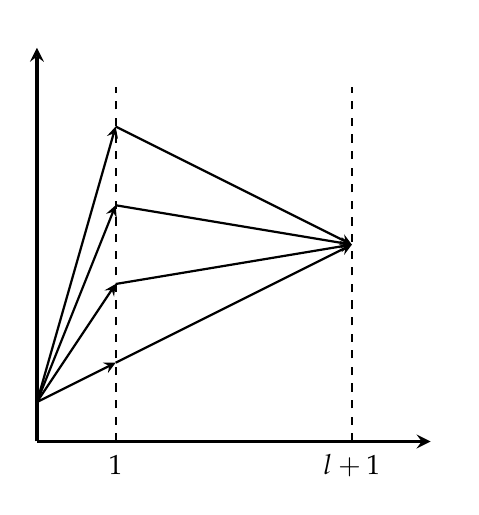
\begin{tikzpicture}

% Axes
\draw[-stealth, very thick] (0,0) -- (5,0) node[right] {};
\draw[-stealth, very thick] (0,0) -- (0,5) node[above] {};

% Vertical dashed lines at k and k+1
\draw[dashed, thick] (1,0) -- (1,4.5);
\draw[dashed, thick] (4,0) -- (4,4.5);


% Arrows from (0,0) to nodes at k
\draw[thick, -stealth] (0,0.5) -- (1,1);
\draw[thick, -stealth] (0,0.5) -- (1,2);
\draw[thick, -stealth] (0,0.5) -- (1,3);
\draw[thick, -stealth] (0,0.5) -- (1,4);

% Arrows from nodes at k to k+1
\draw[thick, -stealth] (1,1) -- (4,2.5);
\draw[thick, -stealth] (1,2) -- (4,2.5);
\draw[thick, -stealth] (1,3) -- (4,2.5);
\draw[thick, -stealth] (1,4) -- (4,2.5);

% Labels
\node at (1,-0.3) {$1$};
\node at (4,-0.31) {$l+1$};

\end{tikzpicture}
\end{document}